\documentclass{beamer}
\usepackage[utf8]{inputenc}

\usepackage{utopia} %font utopia imported

\usepackage{multimedia}
\usepackage{media9}
\usetheme{Madrid}
\usecolortheme{default}
\graphicspath{ {./images/} } 

%------------------------------------------------------------
%This block of code defines the information to appear in the
%Title page
\title %optional
{Multimodal Speech Emotion Recognition Using Audio and Text}

% \subtitle{}


\author[Group J] % (optional)
{Group J: Jan Arvin Lapuz, Alyssa Lim, Le Van Nguyen, Ramil Zabala}


\date[Nov 2020] % (optional)
{COMP8240 Applications of Data Science, Nov 2020}

%------------------------------------------------------------
%The next block of commands puts the table of contents at the 
%beginning of each section and highlights the current section:

\AtBeginSection[]
{
  \begin{frame}
    \frametitle{Presentation Outline}
    \tableofcontents[currentsection]
  \end{frame}
}
%------------------------------------------------------------

\begin{document}

\frame{\titlepage}

%---------------------------------------------------------
%This block of code is for the table of contents after
%the title page
\begin{frame}
\frametitle{Presentation Outline}
\tableofcontents
\end{frame}

%---------------------------------------------------------

\section{Project Overview and Original Replication Results}

%---------------------------------------------------------

\begin{frame}
\frametitle{Paper Abstract}
\textbf{Paper}:
	\begin{itemize}
 	   \item Multimodal Speech Emotion Recognition Using Audio and Text by Seunghyun Yoon, 	Seokhyun Byun, Kyomin Jung
	    %\item Github link: github.com/david-yoon/multimodal-speech-emotion
 	   \item 2018 IEEE Spoken Language Technology Workshop (SLT)
 	   \item Rank 14 in Computational Linguistics Category on Google Scholar
 	   \item Source code is available on author's Github repository without the pretrained model
	\end{itemize}

\textbf{Four models}: Text only, Audio only, Multimodal, Multimodal-Attention 

\textbf{Processed input data}:
    \begin{itemize}
        \item Speech Data (.npy file): Mel Frequency Crystal Coefficients (MFCC), Prosodic Features
        \item Text Data (.npy file): Word Tokens
        \item Emotion Categories: Angry, Happy, Sad, Neutral
    \end{itemize}
    
\textbf{Set up for Google Colab}:
    \begin{itemize}
        \item tensorflow==1.4; python==2.7
        \item scikit-learn==0.20.0; nltk==3.3
        
    \end{itemize}
\end{frame}


% \section{Replication Results}

% \begin{frame}
% \frametitle{Replication Results}
% % \begin{itemize}

% %     \item Results from their original results:
% %     \item Results from our replication
    
    
%     % \item Summary of the previous presentation

% % \end{itemize}

% \begin{center}
%  \begin{tabular}{||c c{1.5cm} c{1.5cm}  ||} 
%  \hline
%  Model & Replication Accuracy & Research Accuracy \\ [0.5ex] 
% % \hspace{5cm} YT \hspace{2cm} TESS \\ [0.5ex] 
%  \hline\hline
%  Text Only  & 0.00\% & 63.5\%  & 62.8\%| \\
%  \hline
%  Audio Only & 51.1\% &  54.6\%   & 62.8\% | \\
%  \hline
%  Multimodal & 0.00\%  & 71.0\%  & 71.8\% | \\
%  Multimodal-Attention & 49.9\% & 69.0\% & 62.8\% | \\

%  \hline
% \end{tabular}
% \end{center}

% \end{frame}
%---------------------------------------------------------
\begin{frame}
\frametitle{Original Replication Results}
 \textbf{Replication of the Original Data (IEMOCAP data)}      

            \begin{center}
                \begin{tabular}{||c c c||} 
                 \hline
                 Model & Published Acc  & Replication Acc\\ [0.2ex] 
                 \hline\hline
                 Text Only & 63.5\% & 62.8\%\\ 
                 \hline
                 Audio Only & 54.6\%  &   55.7\%\\
                 \hline
                 Multimodal & 71.8\% & 71.0\%\\
                 \hline
                 Multimodal-Attention & 69.0\%  & 48.5\%\\
                 \hline
                \end{tabular}
            \end{center}
 
% \textbf{ }   
\end{frame}
%---------------------------------------------------------

\section{New Data Collection and Annotation}

%---------------------------------------------------------

\begin{frame}
\frametitle{Data Collection: YouTube}
% \textbf{Environment}: Google Colab

% \textbf{Requirements}:
\textbf{Approach 1}: YouTube
\begin{itemize}
\item Data Sources:
    \begin{itemize}
    	 \item Dying Young Trailer \url{https://www.youtube.com/watch?v=A8p0w_Ec1NY/}	
    	 \item Trailers of Top 5 romance movies of all time \url{https://www.youtube.com/watch?v=y0F_JE-dSxg/}
     	 \item UNTUCKED: Rupaul's Drag Race S09 E04 \url{https://www.youtube.com/watch?v=6-Eg_TaGfTI/}
    \end{itemize}
\item Audio Extraction:
    \begin{itemize}
    	 \item Used youtube\_dl package in Python	
    	 \item Converted from mp3 to wav using the sox package
    \end{itemize}
\item Transcription:
    \begin{itemize}
    	 \item	Auto-generated captions from YouTube extracted through savesubs.com
    \end{itemize}
\end{itemize}
\end{frame}

% \section{New Data- Youtube Emotion}

\begin{frame}
\frametitle{Data Annotation: YouTube}

Qualtrics Emotion Annotation Survey
\begin{center}
    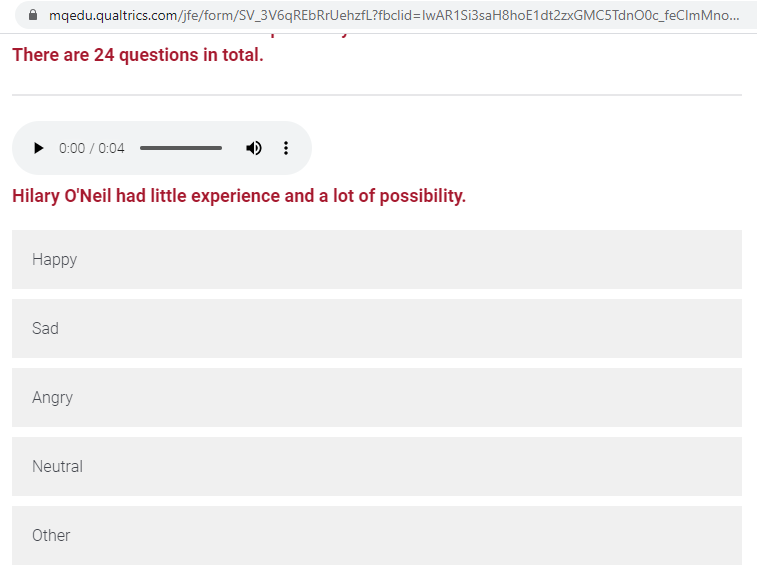
\includegraphics[width=8cm]{images/Qualtrics_Survey.png}
\end{center}
\end{frame}


\begin{frame}
\frametitle{Data Annotation Distribution}


\textbf{YouTube Emotion Distribution}
\\
284 Transcripts Collected in Qualtrics

\begin{center}
    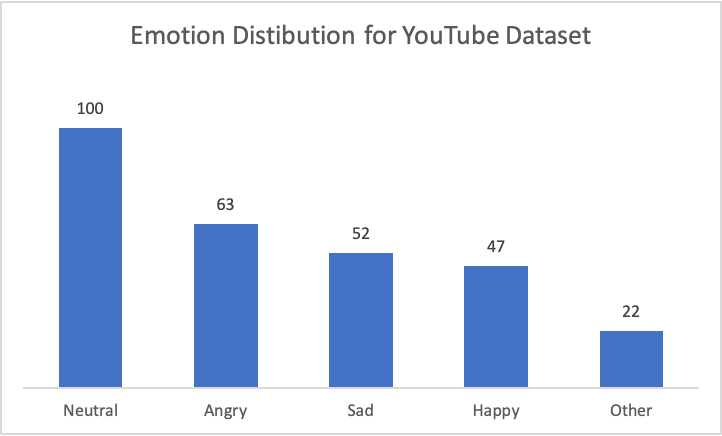
\includegraphics[width=8cm]{images/emo_yt.png}
\end{center}
\end{frame}



% \section{New Data - }

\begin{frame}
\frametitle{Research Data: TESS}
\textbf{Approach 2}: Toronto Emotional Speech Test
\begin{itemize}
\item Audio Description:
    \begin{itemize}
    	 \item	Collected by the University of Toronto, Psychology Department in 2010. There were 200 target words were spoken by two actresses (aged 26 and 64 years) and recordings were made of the set portraying each of seven emotions
    	 \item	Filtered the emotions under category: anger, happiness, sadness, neutral
    \end{itemize}
\item Transcription:
    \begin{itemize}
    	 \item	Google Speech API was used to extract the transcript
    \end{itemize}
\end{itemize}
\end{frame}

\begin{frame}
\frametitle{TESS Emotion Distribution}

\textbf{TESS Emotion Distribution}
\\
8 sets (2 speakers, 4 emotions) with 200 Transcripts each

\begin{center}
    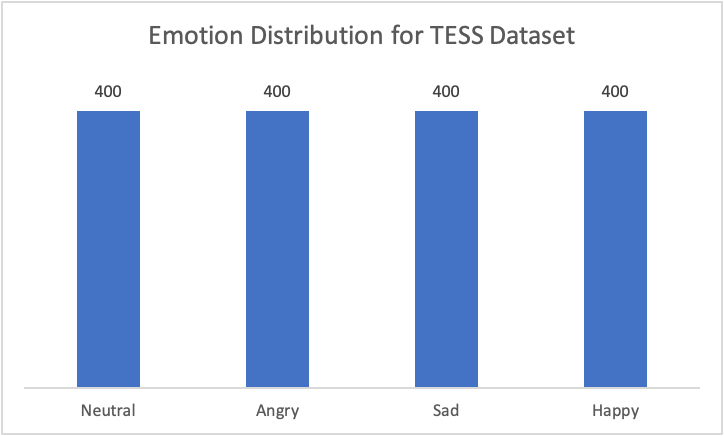
\includegraphics[width=8cm]{images/emo_tess.png}
\end{center}
\end{frame}


% \section{Movie snippet}

% \begin{frame}
% \frametitle{Movie snippet}
% \movie[options]{placeholder box}{images/DY008.wav}
% \movie {images/DY008.wav}

% \includemedia[options]{alt content}{images/DY008.wav}
% \\

% \includemedia[options]{alt content}{images/DY008.wav}
% \\

% \end{frame}

%---------------------------------------------------------

\section{New Data Preprocessing}

%---------------------------------------------------------

\begin{frame}
\frametitle{New Data Preprocessing: Diagram}

\begin{center}
    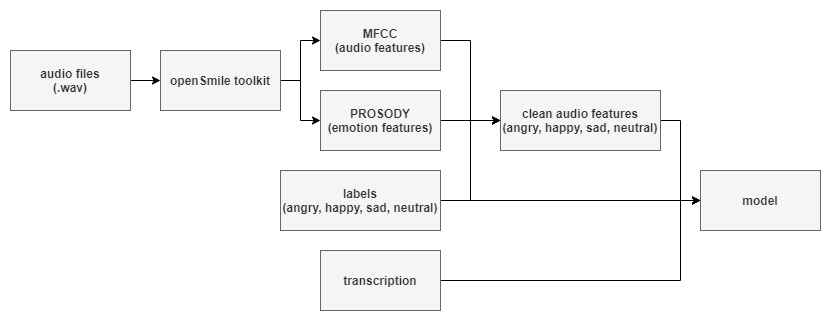
\includegraphics[width=\linewidth,height=\textheight,keepaspectratio]{images/flowchart.jpg}
\end{center}
\end{frame}

\begin{frame}
\frametitle{New Data Preprocessing: Feature Details}
\begin{minipage}{0.4\textwidth}
MFCC (39 Features)
    \begin{itemize}
	    \item Volume 
    	\item Energy 
	    \item Pitch
	    \item Zero Crossing Rate
	    \item Spectral Centroid
	\end{itemize}
\end{minipage}
\begin{minipage}{0.58\textwidth}
    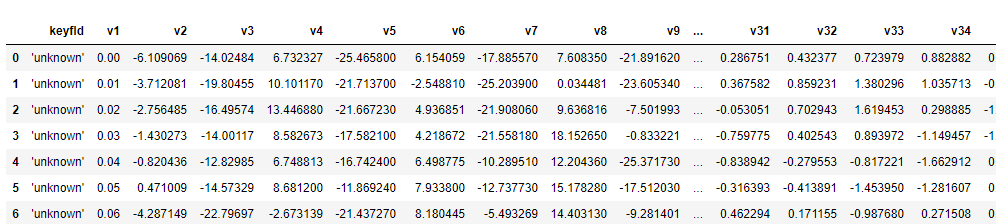
\includegraphics[width=\linewidth,height=\textheight,keepaspectratio]{images/MFCC File Layout.png}
\end{minipage}
\begin{minipage}{0.4\textwidth}
\vspace{.15in}
Prosody (35 Features)
    \begin{itemize}
	    \item Intonation 
    	\item Stress 
	    \item Rhythm
	    \item Speech Rate
	 	\item Pauses
	 	\item Voice Quality	   
	\end{itemize}
\end{minipage}
\begin{minipage}{0.58\textwidth}
    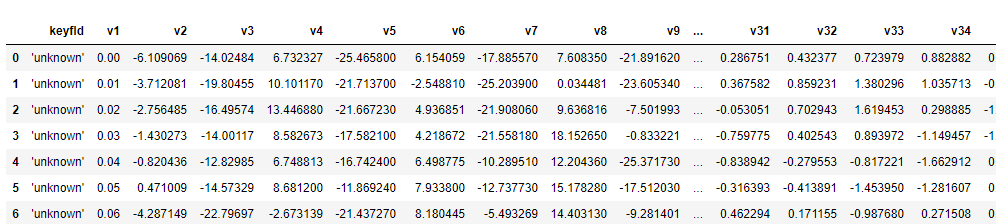
\includegraphics[width=\linewidth,height=\textheight,keepaspectratio]{images/MFCC File Layout.png}
\end{minipage}
\end{frame}


%---------------------------------------------------------

\section{Testing the Model on New Data}

%---------------------------------------------------------
\begin{frame}
\frametitle{Testing the Model on New Data}
% This is a text in second frame. For the sake of showing an example.

\begin{itemize}
    \item Absence of pretrained model
    \item Retraining on original IEMOCAP data - results close to the original 
    \item Training on IEMOCAP data and evaluating the model on the new data (YouTube and TESS)
        \begin{center}
            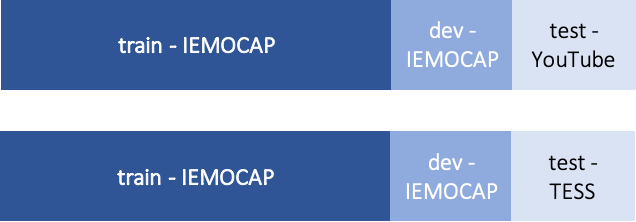
\includegraphics[width=8cm]{images/data_pipeline.png}
        \end{center}
    \item Small modifications to the configuration
\end{itemize}
\end{frame}

%---------------------------------------------------------

\section{Replication Results and Reflection}

%---------------------------------------------------------

\begin{frame}
\frametitle{Replication Results}

    % \begin{itemize}
    %     \item Pre-trained model not available but codes and model parameters are available on GitHub: \href{https://github.com/david-yoon/multimodal-speech-emotion}{https://github.com/david-yoon/multimodal-speech-emotion}
  
  
 \textbf{Replication Results on the Original Data}      

            \begin{center}
                \begin{tabular}{||c c c||} 
                 \hline
                 Model & Published Acc  & Replication Acc\\ [0.2ex] 
                 \hline\hline
                 Text Only & 63.5\% & 62.8\%\\ 
                 \hline
                 Audio Only & 54.6\%  &   55.7\%\\
                 \hline
                 Multimodal & 71.8\% & 71.0\%\\
                 \hline
                 Multimodal-Attention & 69.0\%  & 48.5\%\\
                 \hline
                \end{tabular}
            \end{center}
   
% \textbf{ }     
\textbf{Replication Results on the New Data}    
            \begin{center}
                \begin{tabular}{||c c c||} 
                 \hline
                 Model  & Repl Acc YT   & Repl Acc TESS \\ [0.2ex] 
                 \hline\hline
                 Text Only & 32.7\% & 25.0\% \\ 
                 \hline
                 Audio Only &   23.5\% & 30.6\% \\
                 \hline
                 Multimodal & 27.3\%  & 34.9\%\\
                 \hline
                 Multimodal-Attention & 23.9\%  & 30.8\%\\
                 \hline
                \end{tabular}            
            \end{center}
        %   \begin{center}
        %         \begin{tabular}{||c c{0.5cm} c{0.5cm} c{0.5cm}||} 
        %          \hline
        %          Model & Replication Accuracy TESS  & Replication Accuracy YT  & Research Accuracy \\ [0.2ex] 
        %          \hline\hline
        %          Text Only & 0\% & 62.8\% & 63.5\%\\ 
        %          \hline
        %          Audio Only & 0\% &   55.7\% & 54.6\%\\
        %          \hline
        %          Multimodal & 0\% & 71.0\% & 71.8\%\\
        %          \hline
        %          Multimodal-Attention & 0\% & 48.5\% & 69.0\%\\
        %          \hline
        %         \end{tabular}
        %     \end{center}
    % \end{itemize}

\end{frame}

% \section{Summary and Reflections}

\begin{frame}
\frametitle{Replication Results on Original and New Data}
\begin{center}
    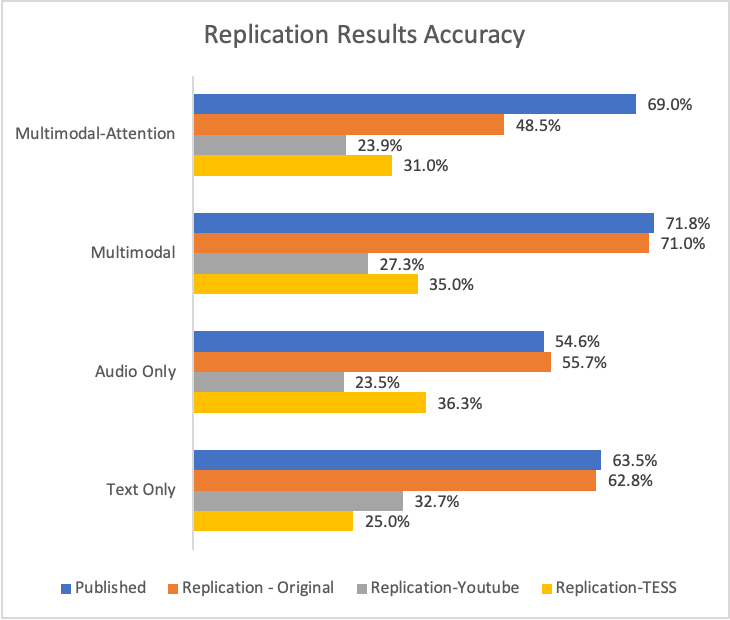
\includegraphics[width=8cm]{images/replication_results.png}
\end{center}
\end{frame}

\begin{frame}[fragile]
  \frametitle{Summary and Reflections}

%   \bigskip

  \begin{itemize}
\item Effect of the TESS dataset variability, i.e., same transcripts spoken in different ways.
 \item	Weight Parameters in openSMILE processing
% suited for IEMOCAP data
% \item The variability of the Tess dataset is not that good because they used the same transcripts for the emotions
\item Effect of background music
\item IEMOCAP data is collected in a controlled environment
% \item 	Small Sample size?


  \end{itemize}


\end{frame}

\end{document}